\documentclass[12pt,letterpaper]{article}
\usepackage[utf8]{inputenc}
\usepackage[spanish]{babel}
\usepackage{graphicx}
\usepackage[left=2cm,right=2cm,top=2cm,bottom=2cm]{geometry}
\usepackage{graphicx} % figuras
% \usepackage{subfigure} % subfiguras
\usepackage{float} % para usar [H]
\usepackage{amsmath}
%\usepackage{txfonts}
\usepackage{stackrel} 
\usepackage{multirow}
\usepackage{enumerate} % enumerados
\renewcommand{\labelitemi}{$-$}
\renewcommand{\labelitemii}{$\cdot$}
% \author{}
% \title{Caratula}
\begin{document}

% Fancy Header and Footer
% \usepackage{fancyhdr}
% \pagestyle{fancy}
% \cfoot{}
% \rfoot{\thepage}
%

% \usepackage[hidelinks]{hyperref} % CREA HYPERVINCULOS EN INDICE

% \author{}
\title{Caratula}

\begin{titlepage}
\begin{center}
\large{UNERSIDAD PRIVADA DE TACNA}\\
\vspace*{-0.025in}
\begin{figure}[htb]
\begin{center}

\includegraphics[width=8cm]{./Imagenes/logo}
\end{center}
\end{figure}
\vspace*{0.15in}
INGENIERIA DE SISTEMAS  \\

\vspace*{0.5in}
\begin{large}
TITULO:\\
\end{large}

\vspace*{0.1in}
\begin{Large}
\textbf{INFORME DE LABORATORIO No 01} \\
\end{Large}

\vspace*{0.3in}
\begin{Large}
\textbf{CURSO:} \\
\end{Large}

\vspace*{0.1in}
\begin{large}
BASE DE DATOS II\\
\end{large}

\vspace*{0.3in}
\begin{Large}
\textbf{DOCENTE(ING):} \\
\end{Large}

\vspace*{0.1in}
\begin{large}
 Patrick Cuadros Quiroga\\
\end{large}

\vspace*{0.2in}
\vspace*{0.1in}
\begin{large}
Integrantes: \\
\begin{flushleft}
Jhony Mamani Limache		\hfill	(2013046566) \\
Colque Ticona Carlos 		\hfill	(2013046500) \\
Luis Zavala Venegas            	\hfill	(2010037899) \\
Moreno C\'aceres Renzo      	\hfill	(2013047246) \\
Ronald Ordoñez Quilli  		\hfill	(2015052821) \\
Condori Tito Hernan  		\hfill	(2009034553) \\
\end{flushleft}
\end{large}
\end{center}

\end{titlepage}


\tableofcontents % INDICE
\thispagestyle{empty} % INDICE SIN NUMERO
\newpage
\setcounter{page}{1} % REINICIAR CONTADOR DE PAGINAS DESPUES DEL INDICE

\section{Actividad No 01 – Revisi\'on de Sintaxis} 
De los siguientes comandos ¿Cuál es el resultado? ¿En caso de ser error cual sería la sentencia correcta?

\begin{itemize}
	\item SELECT last\_name, job\_id, salary AS Sal FROM employees;
	\\Es correcta
	\begin{center}
	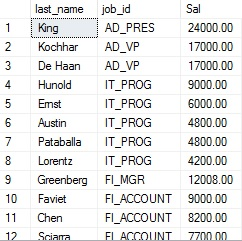
\includegraphics[width=5cm]{./Imagenes/actividad0101} 
	\end{center}

	\item SELECT * FROM job\_grades;
	\\Es incorrecta, la sentencia correcta sería:
	\\SELECT * FROM jobs;
	\begin{center}
	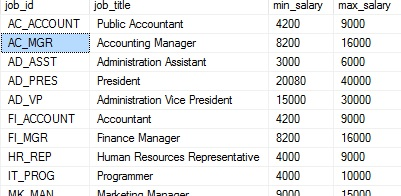
\includegraphics[width=5cm]{./Imagenes/actividad0102} 
	\end{center}
	
	\item SELECT employee\_id, last\_name sal x 12 ANNUAL SALARY FROM employees;
	\\Es incorrecta, la sentencia correcta sería:
	\\SELECT employee\_id, last\_name, salary * 12 'ANNUAL SALARY' FROM employees;
	\begin{center}
	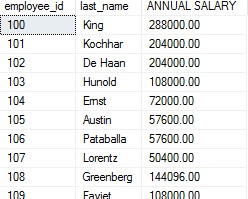
\includegraphics[width=5cm]{./Imagenes/actividad0103} 
	\end{center}

\end{itemize} 
\section{Actividad No 02 – Reconociendo la estructura} 

\begin{enumerate}[1.]
	\item Se requiere determinar la estructura de la tabla DEPARTMENTS y sus datos.
	\\
	\\SP\_HELP 'DEPARTMENTS'

	\begin{center}
	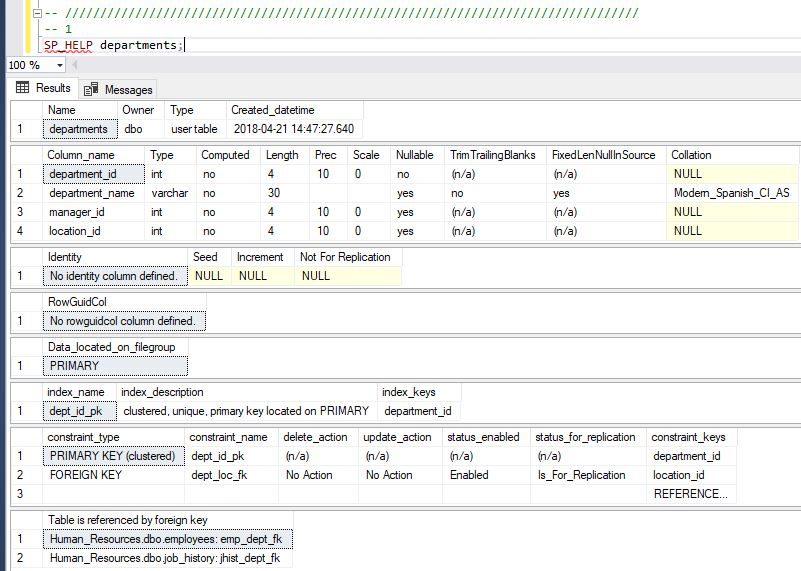
\includegraphics[width=10cm]{./Imagenes/actividad0201} 
	\end{center}

	\item El departamento de Recursos Humanos requiere un reporte que muestre los campos: employee\_id, last\_name y job\_id, asicomo el campo hire\_date con el alias StartDate.

	\begin{center}
	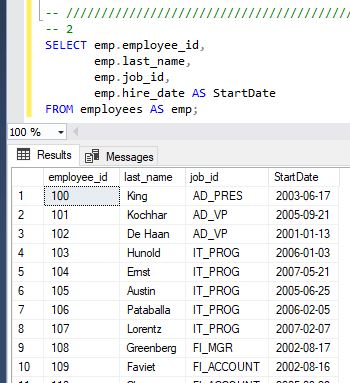
\includegraphics[width=5cm]{./Imagenes/actividad0202} 
	\end{center}

	\item Finalmente el departamento de Recursos Humanos requiere un listado de todos valores del campo JOB\_ID de la tabla EMPLOYEES pero que se muestren de forma única y no repetida.

	\begin{center}
	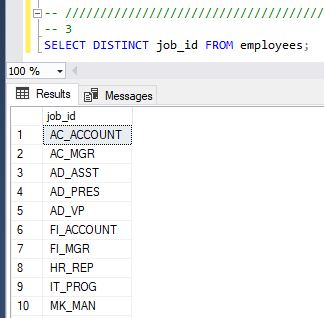
\includegraphics[width=5cm]{./Imagenes/actividad0203} 
	\end{center}

\end{enumerate}



\section{Actividad No 03 – Consultas B\'asicas} 
		
\begin{enumerate}[1.]
	\item El departamento de Recursos Humanos requiere ampliar el reporte anterior (4.2.2) para hacerlo m\'as comprensible, por lo que se requiere que los encabezados de las columnas sean: Emp No, Empleado, Puesto y Fecha Contrataci\'on.

	\begin{center}
	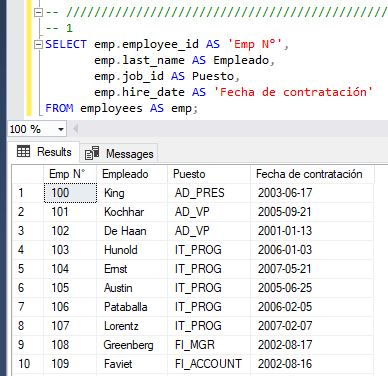
\includegraphics[width=5cm]{./Imagenes/actividad0301} 
	\end{center}

	\item Adicionalmente el departamento de Recursos Humanos requiere un reporte más sencillo, en el que se muestre los campos: last\_name y job\_id en una sola y \'unica columna (los datos deben estar separados por una coma) que tenga como alias Empleado y Puesto.

	\begin{center}
	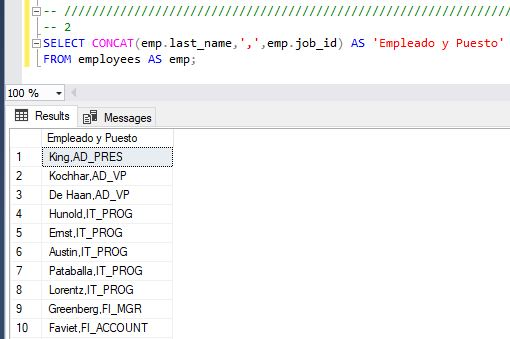
\includegraphics[width=5cm]{./Imagenes/actividad0302} 
	\end{center}

	\item Finalmente a modo de práctica, realizar una consulta que muestre todos los campos de la tabla EMPLOYEES, en una sola y única columna, los datos deben estar separados por una coma y la columna debe tener como encabezado Los Empleados

	\begin{center}
	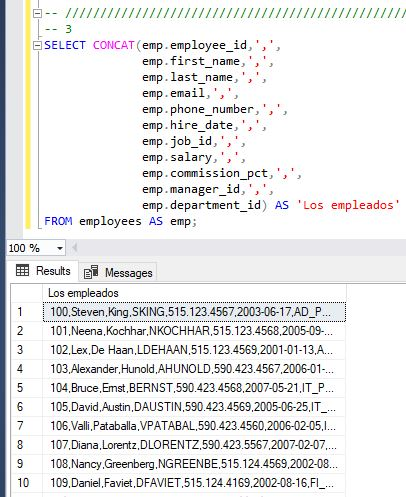
\includegraphics[width=5cm]{./Imagenes/actividad0303} 
	\end{center}

\end{enumerate}




\section{Actividad No 04 – Restricci\'on y Ordenamiento} 
		
\begin{enumerate}[1.]
	\item Debido a problemas con el presupuesto, el departamento de Recursos Humanos requiere un reporte que muestre los apellidos (last\_name) y salarios (salary) de todos los empleados que ganen más de \$ 12,000.
	\\ \\ select last\_name,salary from employees where salary > 12000;

	\begin{center}
	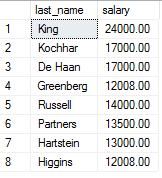
\includegraphics[width=5cm]{./Imagenes/actividad_04_01} 
	\end{center}

	\item Asimismo se requiere realizar una consulta que muestre los apellidos (last\_name) y el n\'umero de departamento (department\_id) para los empleados que tengan numero (employee\_id) 176.
	\\ \\select last\_name,department\_id from employees where employee\_id > 176;

	\begin{center}
	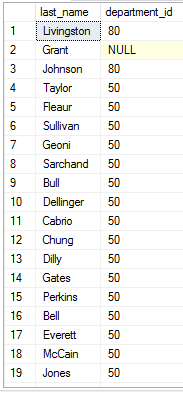
\includegraphics[width=5cm]{./Imagenes/actividad_04_02} 
	\end{center}

	\item El departamento de Recursos Humanos necesita determinar los mayores y menores sueldos, modificar la consulta del  ítem 4.1. para mostrar el apellido y salario de cada empleado cuyo sueldo no est\'e en el rango de \$ 5,000 a \$ 12,000.
	\\ \\select last\_name,job\_id,salary as Sal from employees where salary > 5000 and salary < 12000;

	\begin{center}
	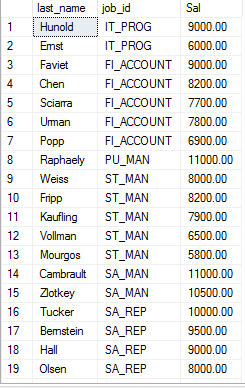
\includegraphics[width=5cm]{./Imagenes/actividad_04_03} 
	\end{center}

	\item Crear un reporte que muestre los apellidos (last\_name), puesto (job\_id) y fecha de contrataci\'on (hire\_date), de los empleados que apellidan ‘Matos’ y ‘Taylor’, asimismo presentar el reporte ordenado ascendentemente por fecha de contrataci\'on.
	\\ \\select last\_name,job\_id,hire\_date from employees where last\_name = 'Matos' or last\_name = 'Taylor' order by hire\_date asc;

	\begin{center}
	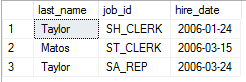
\includegraphics[width=5cm]{./Imagenes/actividad_04_04} 
	\end{center}

	\item Mostrar los apellidos (last\_name) y n\'umero de departamento (departamento\_id) de todos los empleados que pertenezcan a los departamentos 20 o 50 en orden alfab\'etico ascendente por el apellido.
	\\ \\select last\_name,department\_id from employees where department\_id = 20 or department\_id = 50 order by last\_name asc;
	
	\begin{center}
	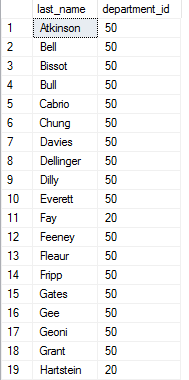
\includegraphics[width=5cm]{./Imagenes/actividad_04_05} 
	\end{center}
	
	\item Modificar el reporte del ítem 4.1. para mostrar los apellidos y salarios de los empleados que tengan un salario entre los \$ 5,000 a \$ 12,000 y pertenezcan a los números de departamento 20 o 50. Asimismo etiquetar las cabeceras de los resultados con los alias Empleado y Salario Mensual respectivamente.
	\\ \\select last\_name 'Empleado',salary 'Salario Mensual' from employees where salary > 5000 and salary < 12000 and (department\_id = 20 or department\_id = 50);

	\begin{center}
	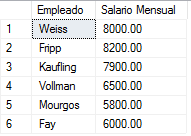
\includegraphics[width=5cm]{./Imagenes/actividad_04_06} 
	\end{center}

	\item El departamento de Recursos Humanos necesita un listado de apellidos (last\_name) y fecha de contrataci\'on (hire\_date) de todos los empleados que fueron contratados el año 1994.
	\\ \\select last\_name,hire\_date from employees where hire\_date between '19940101' and '19941231';

	\begin{center}
	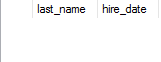
\includegraphics[width=5cm]{./Imagenes/actividad_04_07} 
	\end{center}

	\item Crear un reporte que muestre los apellidos (last\_name) y puesto (job\_id) de todos los empleados que no tengan un administrador (manager).
	\\ \\select last\_name,job\_id from employees where manager\_id is null;

	\begin{center}
	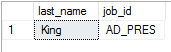
\includegraphics[width=5cm]{./Imagenes/actividad_04_08} 
	\end{center}

	\item Crear un reporte para mostrar los apellidos (last\_name), salario (salary) y \% de comisión (commission\_pct). Ordenar los datos por salario y comisión de manera descendente, utilizar la opción numérica de la cláusula ORDER BY.
	\\ \\select last\_name,salary,commission\_pct from employees order by salary desc,commission\_pct desc;

	\begin{center}
	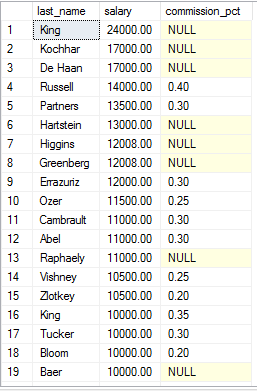
\includegraphics[width=5cm]{./Imagenes/actividad_04_09} 
	\end{center}


	\item El personal del departamento de Recursos Humanos desea tener mayor flexibilidad con los reportes hechos. Por ejemplo se requiere un reporte de los apellidos (last\_name) y salarios (salary) de todos los empleados que tengan un salario mayor a un monto que el personal de Recursos Humanos ingresará. Probar con el valor \$ 12,000.
	\\ \\declare @salario as decimal(9,2); set @salario = 12000; select last\_name,salary from employees where salary > @salario;

	\begin{center}
	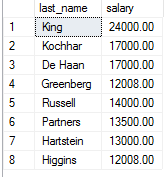
\includegraphics[width=5cm]{./Imagenes/actividad_04_10} 
	\end{center}

	\item El departamento de Recursos Humanos requiere extraer reporte basados en el Administrador (manager\_id). Se requiere crear una consulta que pregunte al usuario por el Administrador (manager\_id) y genere un reporte con los números de empleado (employee\_id), apellidos (last\_name), salarios (salary) y numero de departamento de los empleados que este Administrador tiene a su cargo. Adicionalmente también se desea tener la habilidad de ordenar este reporte en base a una determinada columna. Probar con los siguientes valores:
	\\Administrador (manager\_id) = 103, ordenado por Apellido (last\_name)
	\\Administrador (manager\_id) = 201, ordenado por Salario (salary)
	\\Administrador (manager\_id) = 124, ordenado por No de Empleado (employee\_id)
	\\ \\declare @gerente as int; set @gerente = 103;
	\\select employee\_id,last\_name,salary,department\_id 
	\\from employees where manager\_id = @gerente order by last\_name; 
	\\set @gerente = 201; select employee\_id,last\_name,salary,department\_id 
	\\from employees where manager\_id = @gerente order by salary; 
	\\set @gerente = 124; select employee\_id,last\_name,salary,department\_id 
	\\from employees where manager\_id = @gerente order by employee\_id;

	\begin{center}
	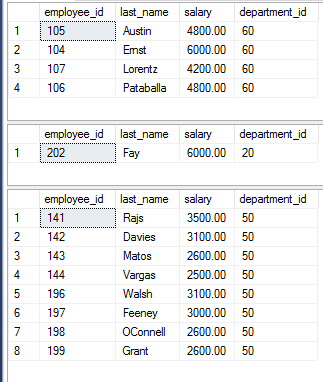
\includegraphics[width=5cm]{./Imagenes/actividad_04_11} 
	\end{center}

	\item Generar un listado de apellidos (last\_name) de todos los empleados que tengan la letra ‘a’ en la tercera letra de su apellido.

	\begin{center}
	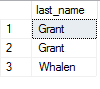
\includegraphics[width=5cm]{./Imagenes/actividad_04_12} 
	\end{center}

	\item Mostrar los apellidos (last\_name) de todos los empleados que tengan tanto la letra ‘a’ como la letra ‘e’
en su apellido.

	\begin{center}
	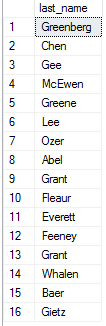
\includegraphics[width=5cm]{./Imagenes/actividad_04_13} 
	\end{center}

	\item Mostrar los apellidos (last\_name), puestos (job\_id) y salario (salary) de todos los empleados que sean Representantes de Ventas (SA\_REP) o Responsables de Inventario (ST\_CLERK) y cuyos salarios no sean iguales a \$ 2,500, \$ 3,500 o \$ 7,000.

	\begin{center}
	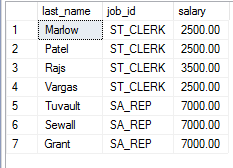
\includegraphics[width=5cm]{./Imagenes/actividad_04_14} 
	\end{center}

	\item Modificar el reporte del ítem 4.6 y mostrar adicionalmente los datos de comisión (commission\_pct) de
todos los empleados que solamente el 20\% de comisi\'on.

	\begin{center}
	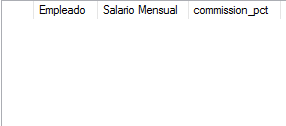
\includegraphics[width=5cm]{./Imagenes/actividad_04_15} 
	\end{center}

\end{enumerate}


% \section{Actividad No 05 – Funciones}
	
\begin{enumerate}[1.]
	\item Se requiere realizar una consulta que visualice la fecha del sistema.
	\\
	\\SELECT CONVERT (date, SYSDATETIME())
	\\,CONVERT (date, SYSDATETIMEOFFSET())
	\\,CONVERT (date, SYSUTCDATETIME())
	\\,CONVERT (date, CURRENT\_TIMESTAMP)
	\\,CONVERT (date, GETDATE())
    	\\,CONVERT (date, GETUTCDATE());
	\begin{center}
	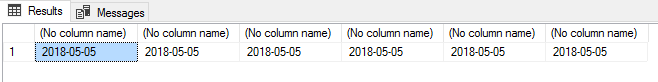
\includegraphics[width=5cm]{./Imagenes/actividad_05_01}
	\end{center}
	
	\item El departamento de Recursos Humanos necesita un reporte de todos los empleados que muestre el No de Empleado, Apellidos, Salario y una columna más con el cálculo del salario incrementado en 15.5\% (expresado solo en enteros) esta columna debe etiquetarse Nuevo Salario
	\\
	\\SELECT employee\_id,last\_name,salary,salary*0.155 as newsalary FROM employees
	\begin{center}
	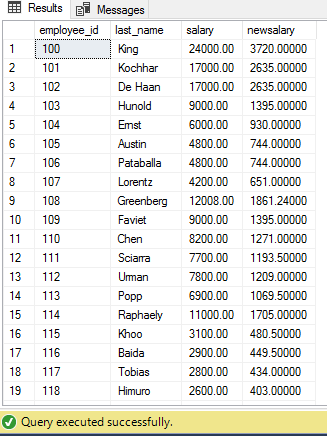
\includegraphics[width=5cm]{./Imagenes/actividad_05_02}
	\end{center}

	\item Modificar la consulta anterior y adicionar una columna que muestre el resultado de la resta entre el antiguo salario y el nuevo salario. Etiquetar esta columna como Incremento.
	\\
	\\SELECT employee\_id,last\_name,salary,salary*0.155 as newsalary,salary-(salary*0.155) as incremento FROM employees
	\begin{center}
	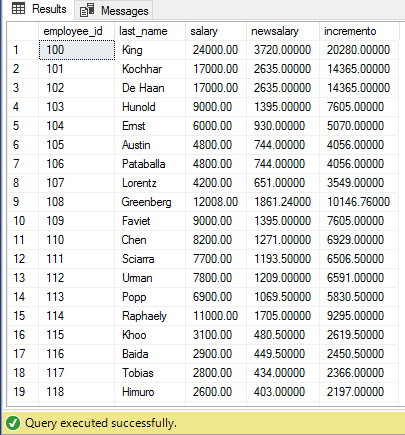
\includegraphics[width=5cm]{./Imagenes/actividad_05_03}
	\end{center}

	\item Crear un reporte que muestre los Apellidos (con la primera letra en May\'usculas y las demás en Min\'usculas) y la longitud de los apellidos (colocar alias Longitud), para todos aquellos empleados quienes sus apellidos empiecen con las letras ‘J’, ‘A’ y ‘M’. Ordenar los resultados por la columna Apellido.
	\\
	\\select UPPER(last\_name) "Apellido", (LOWER(first\_name)) "Longitud" 
	\\from employees 
	\\where last\_name like 'A\%'
     	\\ or last\_name like 'J\%'
      	\\or last\_name like 'M\%' order by last\_name asc;
      	\begin{center}
	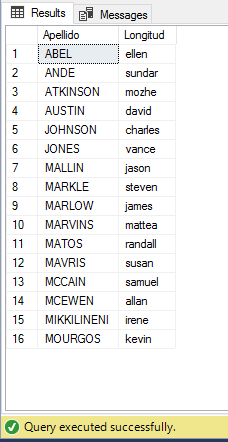
\includegraphics[width=5cm]{./Imagenes/actividad_05_04}
	\end{center}

	\item Modificar la consulta anterior a fin de que consulte primero al usuario con que letra empieza el apellido a buscar. Considerar que no importa si la letra esta may\'uscula o min\'uscula de igual manera debe mostrar los resultados.
	\\
	\\select initcap(FIRST\_NAME) as "name", length(first\_name) as "Length" from employees where upper(substr(first\_name,1,1))=upper('\&Inicial') order by first\_name;

	\item El departamento de Recursos Humanos la duración o tiempo de permanencia de cada empleado, mostrar el Apellido y el calculo del número de meses entre la fecha de hoy y la fecha en que fue contratado el empleado, Etiquetar la columna como Meses Trabajados, ordenar los resultados por el resultado de los n\'umeros de meses, Redondear el número de meses al entero más cercano.
	\\
	\\SELECT LAST\_NAME, ROUND(MONTHS\_BETWEEN(SYSDATE,HIRE\_DATE),0) "MONTHS\_WORKED"
	\\from employees order by MONTHS\_BETWEEN( HIRE\_DATE, SYSDATE);

	\item Crear una consulta que devuelva los Apellidos y Salarios de todos los empleados, Formatear la columna salario para que muestre 15 caracteres, completar con el símbolo ‘\$’ los espacios previos al valor de la columna salario, ejemplo: \$\$\$\$\$\$\$\$\$\$10000. Etiquetar esta columna como Salario.
	\\
	\\CREATE FUNCTION LPAD
	\\(
	\\ @string VARCHAR(MAX), 
	\\@length INT,          
	\\@pad CHAR             
	\\)
	\\RETURNS VARCHAR(MAX)
	\\AS
	\\BEGIN
	    \\RETURN REPLICATE(@pad, @length - LEN(@string)) + @string;
	\\END
	\\GO
	\\SELECT dbo.LPAD(salary, 15, '\$') VALUE
	\\FROM employees;
	\begin{center}
		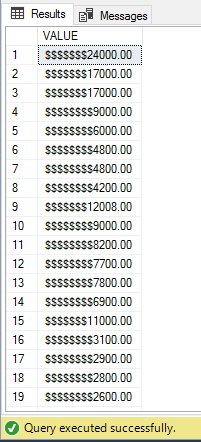
\includegraphics[width=5cm]{./Imagenes/actividad_05_07}
	\end{center}

	\item Crear una consulta que muestre en una única columna los primeros 8 caracteres del apellido de los empleados e indique sus salarios representados por asteriscos (‘*’), cada asterisco representa el valor 1000. Ordenar el listado por el salario de los empleados. Asimismo Etiquetar la columna como ‘Empleados y sus Salarios’.
	\item Finalmente crear una consulta que muestre los Apellidos de los empleados y el No de Semanas Empleado hasta la actualidad para todos los empleados del departamento No 90, truncar el número de semanas a sin decimales. Ordenar el resultado por el No de Semanas y etiquetar la columna como tenencia.
	\\
	\\select last\_name, TRUNC(((SYSDATE-hire\_date)/7),0) as TENURE from employees where department\_id=90 ORDER BY hire\_date DESC;
\end{enumerate}


% \section{Actividad No 06 – Funciones de Conversi\'on} 
		
\begin{enumerate}[1.]
	\item Crear un reporte que muestre lo siguiente por cada empleado.
	\\(Apellido del empleado) gana (Salario) pero quisiera (3 veces Salario).
	\\Etiquetar la columna como Sueldos Soñados.
	\\
	\\select 'Sueldos Soñados'=(last\_name + ' gana ' + Cast(salary as varchar(18)) + ' pero 
	\\quisiera ' + Cast((salary * 3) as varchar(18))) 
	\\from dbo.employees
	\\go
	\\
	\begin{center}
	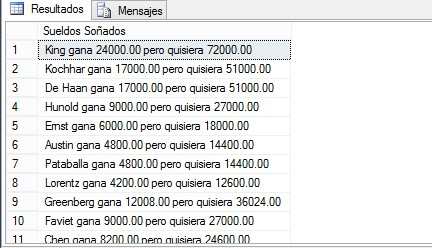
\includegraphics[width=10cm]{./Imagenes/img01} 
	\end{center}

	\item Realizar una consulta que muestre el Apellido del empleado, fecha de contratación y la Fecha de Revisión del Salario, la cual es el primer Lunes después de cada seis meses de servicio, etiquetar la columna como Revisión, asimismo el formato de esta fecha debe ser similar al siguiente: 
	\begin{center}
	Lunes, el veintiuno de julio, 2003 
	\end{center}
	\\
	\\select last\_name, hire\_date as Revision from employees 
	\\where hire\_date between '2003-06-17' and '2005-09-21';
	\\go
	\\
	\begin{center}
	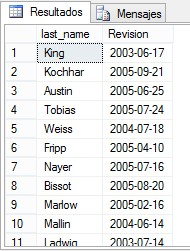
\includegraphics[width=10cm]{./Imagenes/img02} 
	\end{center}

	\item Mostrar un reporte que tenga los Apellidos, Fecha de Contrataci\'on y el D\'ia de Inicio de cada empleado (Lunes, Martes, etc…), etiquetar la \'ultima columna como D\'ia. Ordenar los resultados por el D\'ia de Inicio empezando por Lunes.
	\\
	\\select e.last\_name, e.hire\_date, DateName(WEEKDAY, jh.START\_DATE)as 'Dia' 
	\\from dbo.employees as e inner join dbo.job\_history as jh on 
	\\e.employee\_id=jh.employee\_id
	\\go
	\\
	\begin{center}
	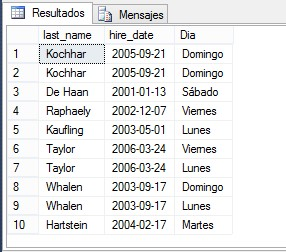
\includegraphics[width=10cm]{./Imagenes/img03} 
	\end{center}

	\item Crear un listado que muestre los Apellidos de los empleados y sus Montos de Comisión, en caso no tenga comisi\'on deber\'a mostrar el texto ‘Sin Comisi\'on’, etiquetar esta ultima columna como Comisi\'on.	
	\\
	\\select last\_name as 'Apellidos', 'Comision'='Sin Comision' from dbo.employees where 
	\\commission\_pct <= 0 
	\\UNION
	\\select last\_name as 'Apellidos', 'Comision'= Cast((salary * commission\_pct) as 	
	\\varchar(20)) from dbo.employees where commission\_pct > 0
	\\go
	\\
	\begin{center}
	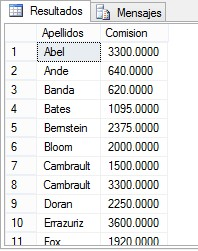
\includegraphics[width=10cm]{./Imagenes/img04} 
	\end{center}

	\item Utilizando la función DECODE, crear un reporte que muestre los apellidos, los puestos y los grados de los empleados basados en sus puestos, utilizando la siguiente información:
	\begin{center}
		\begin{tabular}{ c c }
		Puesto & Grado \\
		\hline
		AD\_PRES & A \\
		ST\_MAN & B \\
		IT\_PROG & C \\
		SA\_REP & D \\
		ST\_CLERK & E \\
		Ninguno de los Anteriores & 0 \\
		\end{tabular}
	\end{center}
	\item Rescribir la consulta anterior utilizando la función CASE.
	\\
	\\select e.last\_name as 'Apellidos', j.job\_title, case 
	\\when j.job\_id = 'AD\_PRES' THEN 'A'
	\\when j.job\_id = 'ST\_MAN' THEN 'B'
	\\when j.job\_id = 'IT\_PROG' THEN 'C'
	\\when j.job\_id = 'SA\_REP' THEN 'D'
	\\else '0' END as 'Grados' from dbo.employees as e inner join dbo.jobs as j on 
	\\e.job\_id=j.job\_id
	\\go
	\\
	\begin{center}
	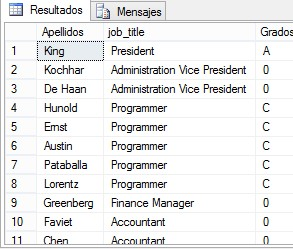
\includegraphics[width=10cm]{./Imagenes/img06} 
	\end{center}
\end{enumerate}


\section{Actividad No 07 – Funciones de Agrupaci\'on} 
		
\begin{enumerate}[1.]
	\item El departamento de Recursos Humanos requiere un reporte que muestre el máximo, el mínimo, la suma y el promedio de los salarios de todos los empleados, Etiquetar esta columnas como Máximo, Mínimo, Suma y Promedio respectivamente, Redondear estos valores a enteros sin decimales.
	\item Modificar la consulta anterior para mostrar el máximo, mínimo, suma y promedio de los salarios por cada Puesto de trabajo. 
	\item Realizar un reporte que muestre la cantidad de empleados por Puesto de trabajo. Con la opción de que el usuario pueda ingresar todos los puestos o uno solo.
	\item Determinar el n\'umero de Administradores o Supervisores utilizar la columna manager\_id para esto. Etiquetar la columna como No de Administradores
	\item Encontrar la diferencia entre el m\'aximo y m\'inimo salario de los empleados. Etiquetar la columna como Diferencia
	\item Crear un reporte que muestre los No de Administradores (manager\_id) y el salario de su empleado peor pagado. Excluir a los empleados cuyo Administrador no se conozca. Excluir asimismo cualquier grupo cuyo salario mínimo sea \$6000 o menos. Ordenar los resultados por el mínimo salario en forma descendente.
	\item Crear una consulta que muestre el número total de empleados, así como el número total de empleados contratados en los años 1995, 1996, 1997 y 1998, etiquetar las columnas apropiadamente.
	\item Crear una consulta matriz que muestre el puesto, el salario por cada puesto basado en el No de Departamento del empleado y el total del salario para cada puesto para los departamento 20, 50, 80 y 90, colocar un nombre apropiado a cada columna.
\end{enumerate}


% \section{Actividad No 08 – Enlaces} 
		
\begin{enumerate}[1.]
	\item El departamento de Recursos Humanos requiere un reporte que muestre las direcciones de todos los departamentos. Utilizar las tablas LOCATIONS y COUNTRIES. Mostrar el ID de la Ubicación (location\_id), dirección (street\_address), ciudad (city), estado o provincia (state\_province) y país (country\_name). % Utilizar NATURAL JOIN para producir el resultado.
	\begin{center}
	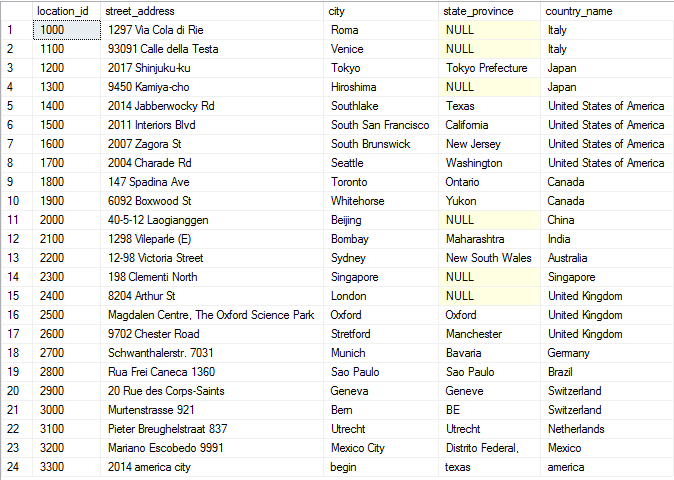
\includegraphics[width=5cm]{./Imagenes/actividad_08_01} 
	\end{center}


	\item El departamento de Recursos Humanos necesita un reporte de todos empleados, que muestres los apellidos de empleado (last\_name), el No de departamento (department\_id) y el nombre del departamento (depertment\_date) al cual pertenece. 

	\begin{center}
	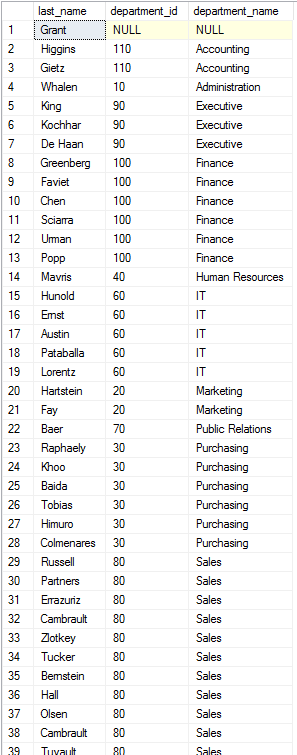
\includegraphics[width=5cm]{./Imagenes/actividad_08_02} 
	\end{center}

	\item El departamento de Recursos Humanos necesita un reporte de los empleados de la ciudad de Toronto. Mostrar los Apellidos, Puesto, No de Departamento y Nombre de Departamento de todos los empleados que trabajan en Toronto.

	\begin{center}
	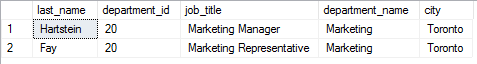
\includegraphics[width=5cm]{./Imagenes/actividad_08_03} 
	\end{center}

	\item Crear un reporte que muestre los Apellidos y No de Identificación de los empleados, asimismo también
debe mostrarse el Apellido y No de Identificaci\'on de su Administrador.

	\begin{center}
	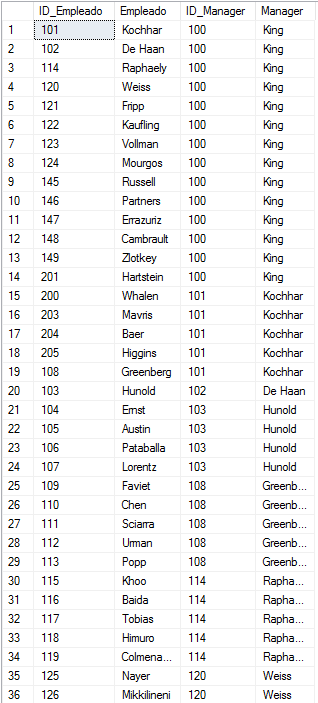
\includegraphics[width=5cm]{./Imagenes/actividad_08_04} 
	\end{center}

	\item Modificar la consulta anterior para que incluya tambi\'en a los empleados quienes no tienen Administrador asignado.

	\begin{center}
	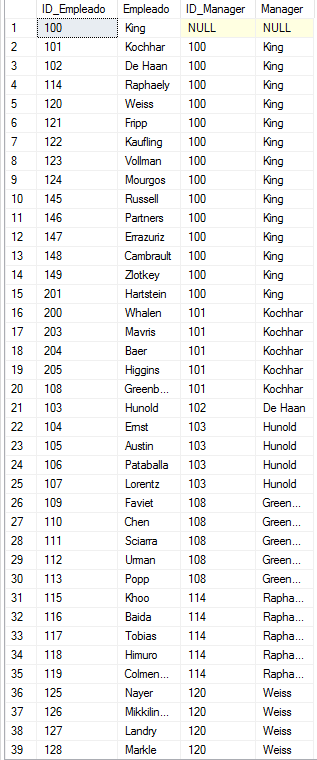
\includegraphics[width=5cm]{./Imagenes/actividad_08_05} 
	\end{center}

	\item Crear un reporte que muestre los No de Departamento y Apellidos de todos los empleados, asimismo adicionar una columna con los Apellidos de todos empleados que trabajan en el mismo departamento. Etiquetar esta columna como Colega.
	\item El departamento de Recursos Humanos requiere un reporte de todo el personal que fue contratado después del empleado apellidado ‘Davies’. Crear un reporte que muestre el apellidos y fecha de contrataci\'on de todo los empleados contratado después de ‘Davies’.
	\item El departamento de Recursos Humanos requiere de un reporte que el apellido del empleado, fecha de contrataci\'on del empleado, apellido del administrador, fecha de contratación del administrador. Para todos aquellos empleados que fueron contratados antes que sus Administradores.
\end{enumerate}


% \section{Actividad No 09 – SubConsultas} 
		
\begin{enumerate}[1.]
	\item El departamento de Recursos Humanos requiere una consulta que pregunte al usuario por el Apellido del empleado, Luego la consulta deber\'a mostrar los Apellidos y Fecha de Contrataci\'on de todos los empleados del mismo departamento excluyendo o con excepción del empleado el cual ha sido proporcionado su apellido reporte que muestre las direcciones de todos los departamentos.
	\\
	\\-- leyendo id de empleado\\
	SET @empid \= 110\\
	-- obteniendo id de departamento de empleado \\
	SET @depid \= (SELECT emp.department\_id \\
	FROM employees as emp \\
	WHERE emp.employee\_id\=@empid); \\
	-- todos los empleados del mismo departamento excluyendo al empleado ingresado anteriormente\\
	SELECT emp.employee\_id, \\
	emp.last\_name, \\
	emp.hire\_date, \\
	emp.department\_id \\
	FROM employees AS emp \\
	WHERE emp.department\_id\=@depid \\
	AND emp.employee\_id!\=@empid; \\
	\begin{center}
	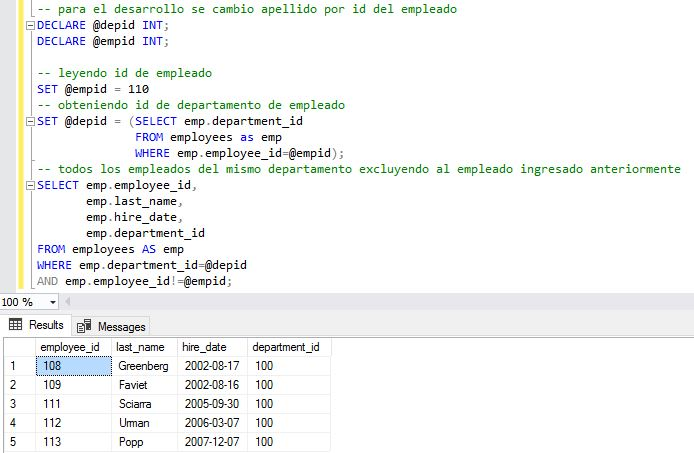
\includegraphics[width=5cm]{./Imagenes/actividad0901} 
	\end{center}

	\item Crear un reporte que muestre el No del Empleado, Apellidos y Salarios de todos los empleados que tienen un salario superior al promedio de salarios de todos los empleados. Ordenar los resultados por el Salario de forma ascendente.
	\\
	\\SELECT emp.employee\_id, \\
	emp.last\_name, \\
	emp.salary \\
	FROM employees AS emp \\
	WHERE emp.salary>@prom; \\
	\begin{center}
	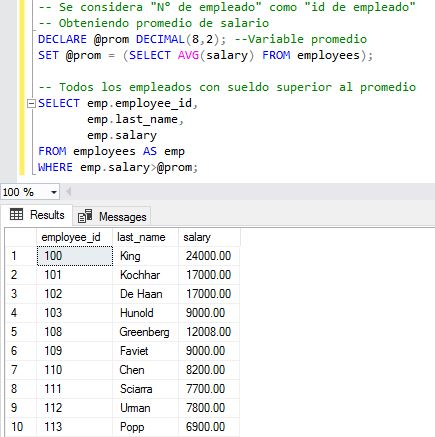
\includegraphics[width=5cm]{./Imagenes/actividad0902} 
	\end{center}

	\item Realizar un reporte que muestre el No de Empleado y Apellidos de todos los empleados quienes trabajan
	\\
	\\SELECT emp.employee\_id, \\
	emp.last\_name, \\
	emp.department\_id \\
	FROM employees AS emp \\
	JOIN (SELECT DISTINCT department\_id \\
		  FROM employees \\
		  WHERE last\_name LIKE '\%u\%') AS depid \\
	ON emp.department\_id\=depid.department\_id; \\
	\begin{center}
	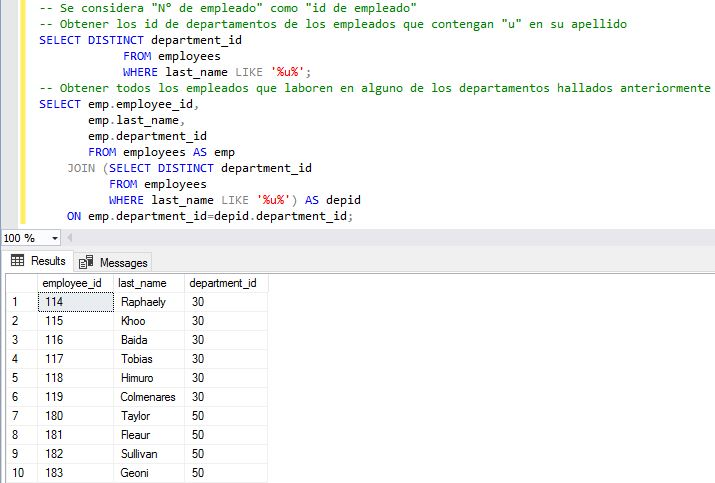
\includegraphics[width=5cm]{./Imagenes/actividad0903} 
	\end{center}

en el departamento de cualquier empleado que su apellido contenga la letra ‘u’.
	\item El departamento de Recursos Humanos requiere un reporte que muestre los Apellidos, No de Departamento y Puestos de los empleados cuya locación de departamento es 1700.
	\\
	\\SELECT emp.last\_name, \\
	emp.department\_id, \\
	dep.location\_id \\
	FROM employees as emp \\
	JOIN departments as dep \\
	ON emp.department\_id\=dep.department\_id \\
	WHERE dep.location\_id\=1700;\\
	\begin{center}
	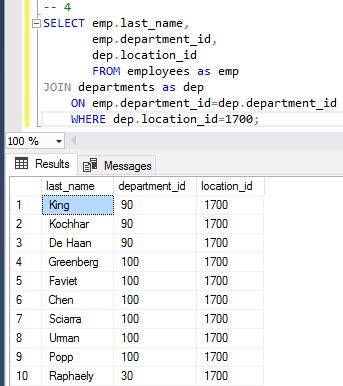
\includegraphics[width=5cm]{./Imagenes/actividad0904} 
	\end{center}

	\item Modificar la consulta anterior de forma que el usuario pueda introducir el No de locaci\'on.
	\\
	\\DECLARE @locid INT; \\
	SET @locid \= 1700; \\
	SELECT emp.last\_name, \\
	   emp.department\_id, \\
	   dep.location\_id \\
	   FROM employees as emp \\
	JOIN departments as dep \\
	ON emp.department\_id\=dep.department\_id \\
	WHERE dep.location\_id\=@locid; \\
	\begin{center}
	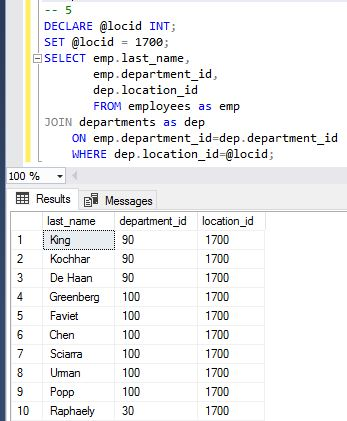
\includegraphics[width=5cm]{./Imagenes/actividad0905} 
	\end{center}

	\item Crear un reporte para el departamento de Recursos Humanos que muestre los Apellidos y Salarios de todos los empleados cuyo Administrador apellide ‘King’.
	\\
	\\SELECT emp.last\_name, \\
	   emp.salary \\
	   FROM employees AS emp \\
JOIN (SELECT dep.department\_id \\
			 FROM departments AS dep \\
	  JOIN (SELECT employee\_id, \\
			       last\_name \\
				   FROM employees \\
				   WHERE last\_name\='KING') AS manking \\
	  ON dep.manager\_id\=manking.employee\_id) AS depking \\
ON emp.department\_id\=depking.department\_id; \\
	\begin{center}
	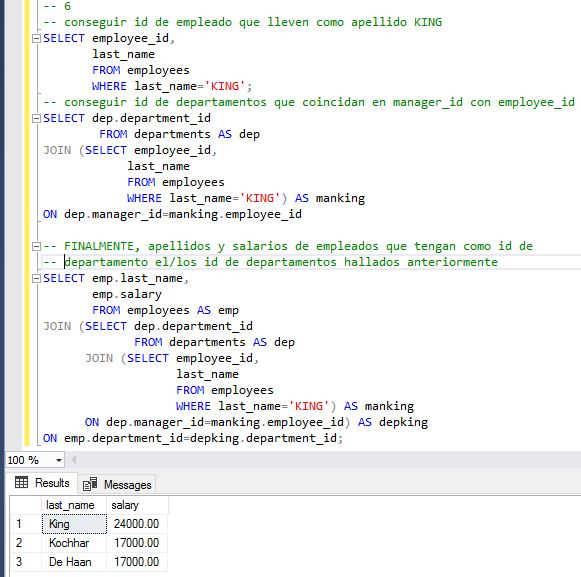
\includegraphics[width=5cm]{./Imagenes/actividad0906} 
	\end{center}

	\item Crear un reporte para el departamento de Recursos Humanos que muestre el No de Departamento, Apellidos, Puestos de todos los empleados en el departamento ‘Executive’.
\\
\\SELECT empnomjob.department\_id, \\
	   empnomjob.last\_name, \\
	   empnomjob.job\_title \\
	   FROM departments \\
JOIN (SELECT emp.department\_id, \\
			 emp.last\_name, \\
			 jobs.job\_title \\
			 FROM employees AS emp \\
	  JOIN jobs \\
	  ON emp.job\_id\=jobs.job\_id) AS empnomjob \\
ON empnomjob.department\_id\=departments.department\_id \\
WHERE department\_name\='executive' \\
	\begin{center}
	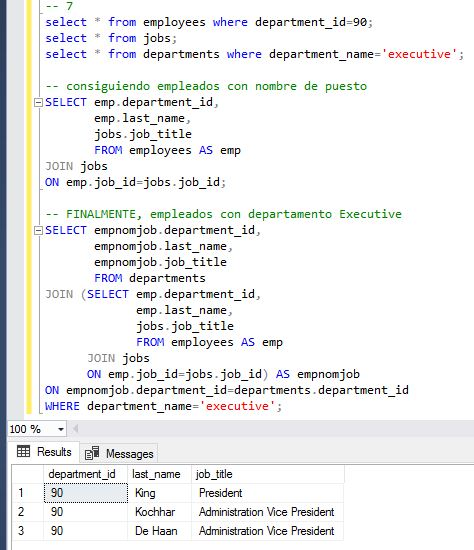
\includegraphics[width=5cm]{./Imagenes/actividad0907} 
	\end{center}

	\item Modificar la consulta del ítem 4.3 para que adicionalmente se muestro solo a los empleados que tengan un salario mayor al promedio de todos los salarios de los empleados.
\end{enumerate}

\section{Actividad No 10 – Conjuntos} 
		
\begin{enumerate}[1.]
	\item El departamento de Recursos Humanos requiere un reporte de todos los departamentos que no contengan un empleado con el puesto ‘ST\_CLERK’. Utilizar el operador MINUS o EXCEPT para esta solicitud.
	\item El departamento de Recursos Humanos requiere adicionalmente una lista de todos los pa\'ises que no tengan un departamento de la empresa localizado en ellos, mostrar el código del país y el nombre. Utilizar el operador MINUS o EXCEPT para realizar esta operaci\'on.
	\item Se necesita una lista de puestos de los departamentos 10, 50 y 20, en ese orden, mostrar el c\'odigo del puesto y c\'odigo del departamento. Utilizar el operador UNION ALL.
	\item Crear un reporte que muestre que liste los c\'odigos de los empleados y los puestos de todos aquellos empleados que tienen el mismo puesto que en el momento en el que fueron contratados por la empresa, cambiaron de puestos y luego volvieron al puesto anterior. Utilizar el operador INTERSECT.
	\item El departamento de Recursos Humanos requiere un reporte que muestre lo siguiente:
	\begin{itemize}
		\item Apellidos y c\'odigos de departamentos de todos los registros de la tabla empleados sin importar si pertenecen a uno o ningún departamento.
		\item C\'odigo de departamentos y nombres de departamentos de la tabla DEPARTAMENTOS inclusive si no existiese ningún empleado en ese departamento
	\end{itemize}
	Ambos requerimientos se deben mostrar en un mismo resultado. Utilizar el operador UNION ALL.
\end{enumerate}



\end{document}
